% Figure 5: Defense Effectiveness Analysis (simulated data)
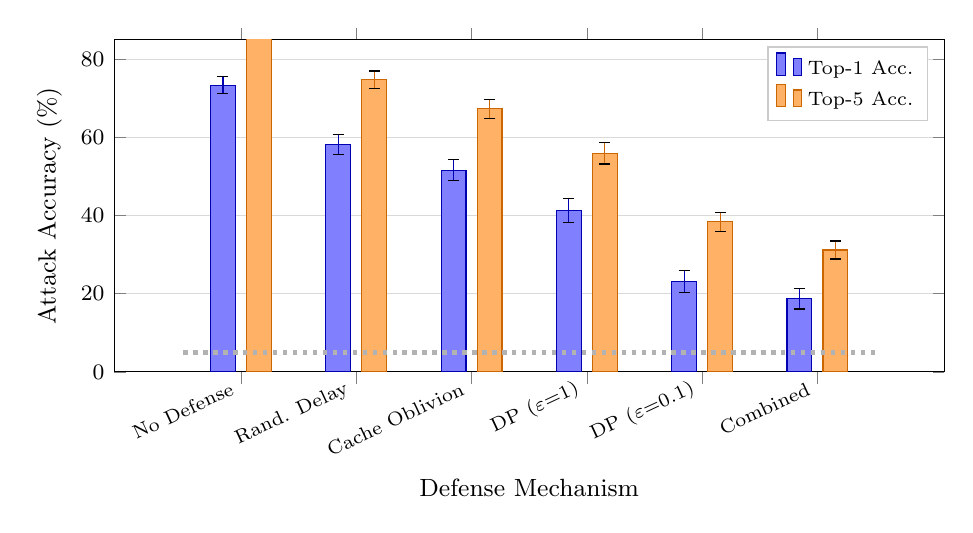
\begin{tikzpicture}
\begin{axis}[
    width=\columnwidth,
    height=5.8cm,
    ybar=4pt,
    bar width=9pt,
    xlabel={Defense Mechanism},
    ylabel={Attack Accuracy (\%)},
    ymin=0, ymax=85,
    ytick={0,20,40,60,80},
    xtick=data,
    xticklabels={No Defense, Rand. Delay, Cache Oblivion, DP ($\varepsilon{=}1$), DP ($\varepsilon{=}0.1$), Combined},
    xticklabel style={font=\scriptsize, rotate=25, anchor=east},
    legend style={at={(0.98,0.98)}, anchor=north east, font=\scriptsize,
                  draw=gray!40, fill=white},
    ymajorgrids=true,
    grid style={line width=0.3pt, draw=gray!30},
    tick label style={font=\footnotesize},
    label style={font=\small},
    legend cell align=left,
]

% Top-1 accuracy under each defense
\addplot[fill=blue!50, draw=blue!70!black,
         error bars/.cd, y dir=both, y explicit]
coordinates {
(1, 73.4) +- (0, 2.1)
(2, 58.2) +- (0, 2.5)
(3, 51.6) +- (0, 2.7)
(4, 41.3) +- (0, 3.0)
(5, 23.1) +- (0, 2.8)
(6, 18.7) +- (0, 2.6)
};
\addlegendentry{Top-1 Acc.};

% Top-5 accuracy under each defense
\addplot[fill=orange!60, draw=orange!80!black,
         error bars/.cd, y dir=both, y explicit]
coordinates {
(1, 91.2) +- (0, 1.4)
(2, 74.8) +- (0, 2.2)
(3, 67.3) +- (0, 2.4)
(4, 55.9) +- (0, 2.7)
(5, 38.4) +- (0, 2.5)
(6, 31.2) +- (0, 2.3)
};
\addlegendentry{Top-5 Acc.};

% Reference line: random guess
\addplot[gray!60, sharp plot, ultra thick, dotted, forget plot]
coordinates {(0.5,5.0) (6.5,5.0)};

\end{axis}
\end{tikzpicture}
